\subsection{Evaluation Metrics and Mathematical Formulations}
Systems are evaluated according to the official shared task criteria and complementary secondary metrics:
\begin{enumerate}
    \item \textbf{Official Subtask 2 Metric}: Macro-averaged positive-class $F_1$ across target lemmas:
    \begin{equation}
    F_{1,\text{official}} = \frac{1}{|W|} \sum_{w=1}^{|W|} F_{1,w}, \quad \text{where } F_{1,w} = \frac{2\text{TP}_w}{2\text{TP}_w + \text{FP}_w + \text{FN}_w}.
    \end{equation}
    Words with zero true positives and zero predicted positives contribute $0.0$.
    \item \textbf{Secondary Classification Metrics}:
    \begin{itemize}
        \item \textit{Pooled Macro-$F_1$}: Standard $F_1$ averaged across both binary classes ($c \in \{0, 1\}$).
        \item \textit{Accuracy}: Fraction of correct instance-level predictions $\frac{\text{TP} + \text{TN}}{N}$.
    \end{itemize}
    \item \textbf{Information Retrieval Ranking Metrics}: Evaluated across the $|Q|=10$ word queries:
    \begin{itemize}
        \item \textit{Mean Reciprocal Rank (MRR)}: $\text{MRR} = \frac{1}{|Q|} \sum_{q=1}^{|Q|} \frac{1}{\text{rank}_q^*}$.
        \item \textit{Mean Average Precision (MAP)}: Mean of average precision over positive docs.
        \item \textit{Normalized Discounted Cumulative Gain at rank 10 (nDCG@10)}.
    \end{itemize}
\end{enumerate}

\subsection{Subtask 2 Benchmark Results Across Random Seeds}
Table~\ref{tab:subtask2_benchmark} presents the multi-seed benchmark performance over the 5 random splits. We report the sample mean ($\mu$), sample standard deviation ($\sigma$), and 95\% bootstrap percentile confidence intervals ($N_{\text{boot}}=1,000$).

\begin{table}[t]
\centering
\small
\begin{tabular}{llcccc}
\toprule
\textbf{Phase} & \textbf{Model / System} & \textbf{Official $F_1$} & \textbf{95\% CI} & \textbf{Pooled $F_1$} & \textbf{Accuracy} \\
\midrule
A1 & Pretrained Baseline & 0.489 $\pm$ 0.022 & [0.473, 0.507] & 0.715 & 0.737 \\
A1 & Trivial Reference & 0.470 $\pm$ 0.018 & [0.455, 0.481] & 0.262 & 0.355 \\
A1 & Ablation Baseline & 0.460 $\pm$ 0.047 & [0.422, 0.495] & 0.748 & 0.766 \\
A1 & Pretrained Baseline & 0.459 $\pm$ 0.023 & [0.441, 0.476] & 0.695 & 0.718 \\
A1 & Classical ML & 0.455 $\pm$ 0.045 & [0.420, 0.491] & 0.798 & 0.822 \\
A1 & Classical ML & 0.450 $\pm$ 0.049 & [0.412, 0.489] & 0.811 & 0.836 \\
A2 & DENSE (Tuned K*=100) & 0.448 $\pm$ 0.016 & [0.434, 0.459] & 0.554 & 0.565 \\
A1 & Classical ML & 0.446 $\pm$ 0.039 & [0.419, 0.478] & 0.801 & 0.823 \\
A2 & HYBRID (Tuned K*=100) & 0.418 $\pm$ 0.029 & [0.395, 0.440] & 0.525 & 0.536 \\
A2 & BM25 (Tuned K*=100) & 0.358 $\pm$ 0.016 & [0.343, 0.367] & 0.481 & 0.491 \\
A1 & Classical ML & 0.341 $\pm$ 0.026 & [0.321, 0.362] & 0.811 & 0.834 \\
A2 & DENSE (Naive K=50) & 0.327 $\pm$ 0.030 & [0.304, 0.350] & 0.537 & 0.612 \\
A2 & HYBRID (Naive K=50) & 0.313 $\pm$ 0.036 & [0.284, 0.341] & 0.521 & 0.598 \\
A2 & BM25 (Naive K=50) & 0.236 $\pm$ 0.027 & [0.214, 0.254] & 0.476 & 0.558 \\
A1 & Classical ML & 0.228 $\pm$ 0.063 & [0.182, 0.277] & 0.600 & 0.723 \\
A1 & Simple Baseline & 0.000 $\pm$ 0.000 & [0.000, 0.000] & 0.392 & 0.645 \\
\bottomrule
\end{tabular}
\caption{Subtask 2 classification benchmark across 5 random seeds (80/20 stratified split, $n_{\text{test}}=397$). Official metric is per-word macro-averaged positive-class $F_1$. Secondary metrics include pooled macro-$F_1$ and accuracy.}
\label{tab:subtask2_benchmark}
\end{table}

\begin{figure}[H]
\centering
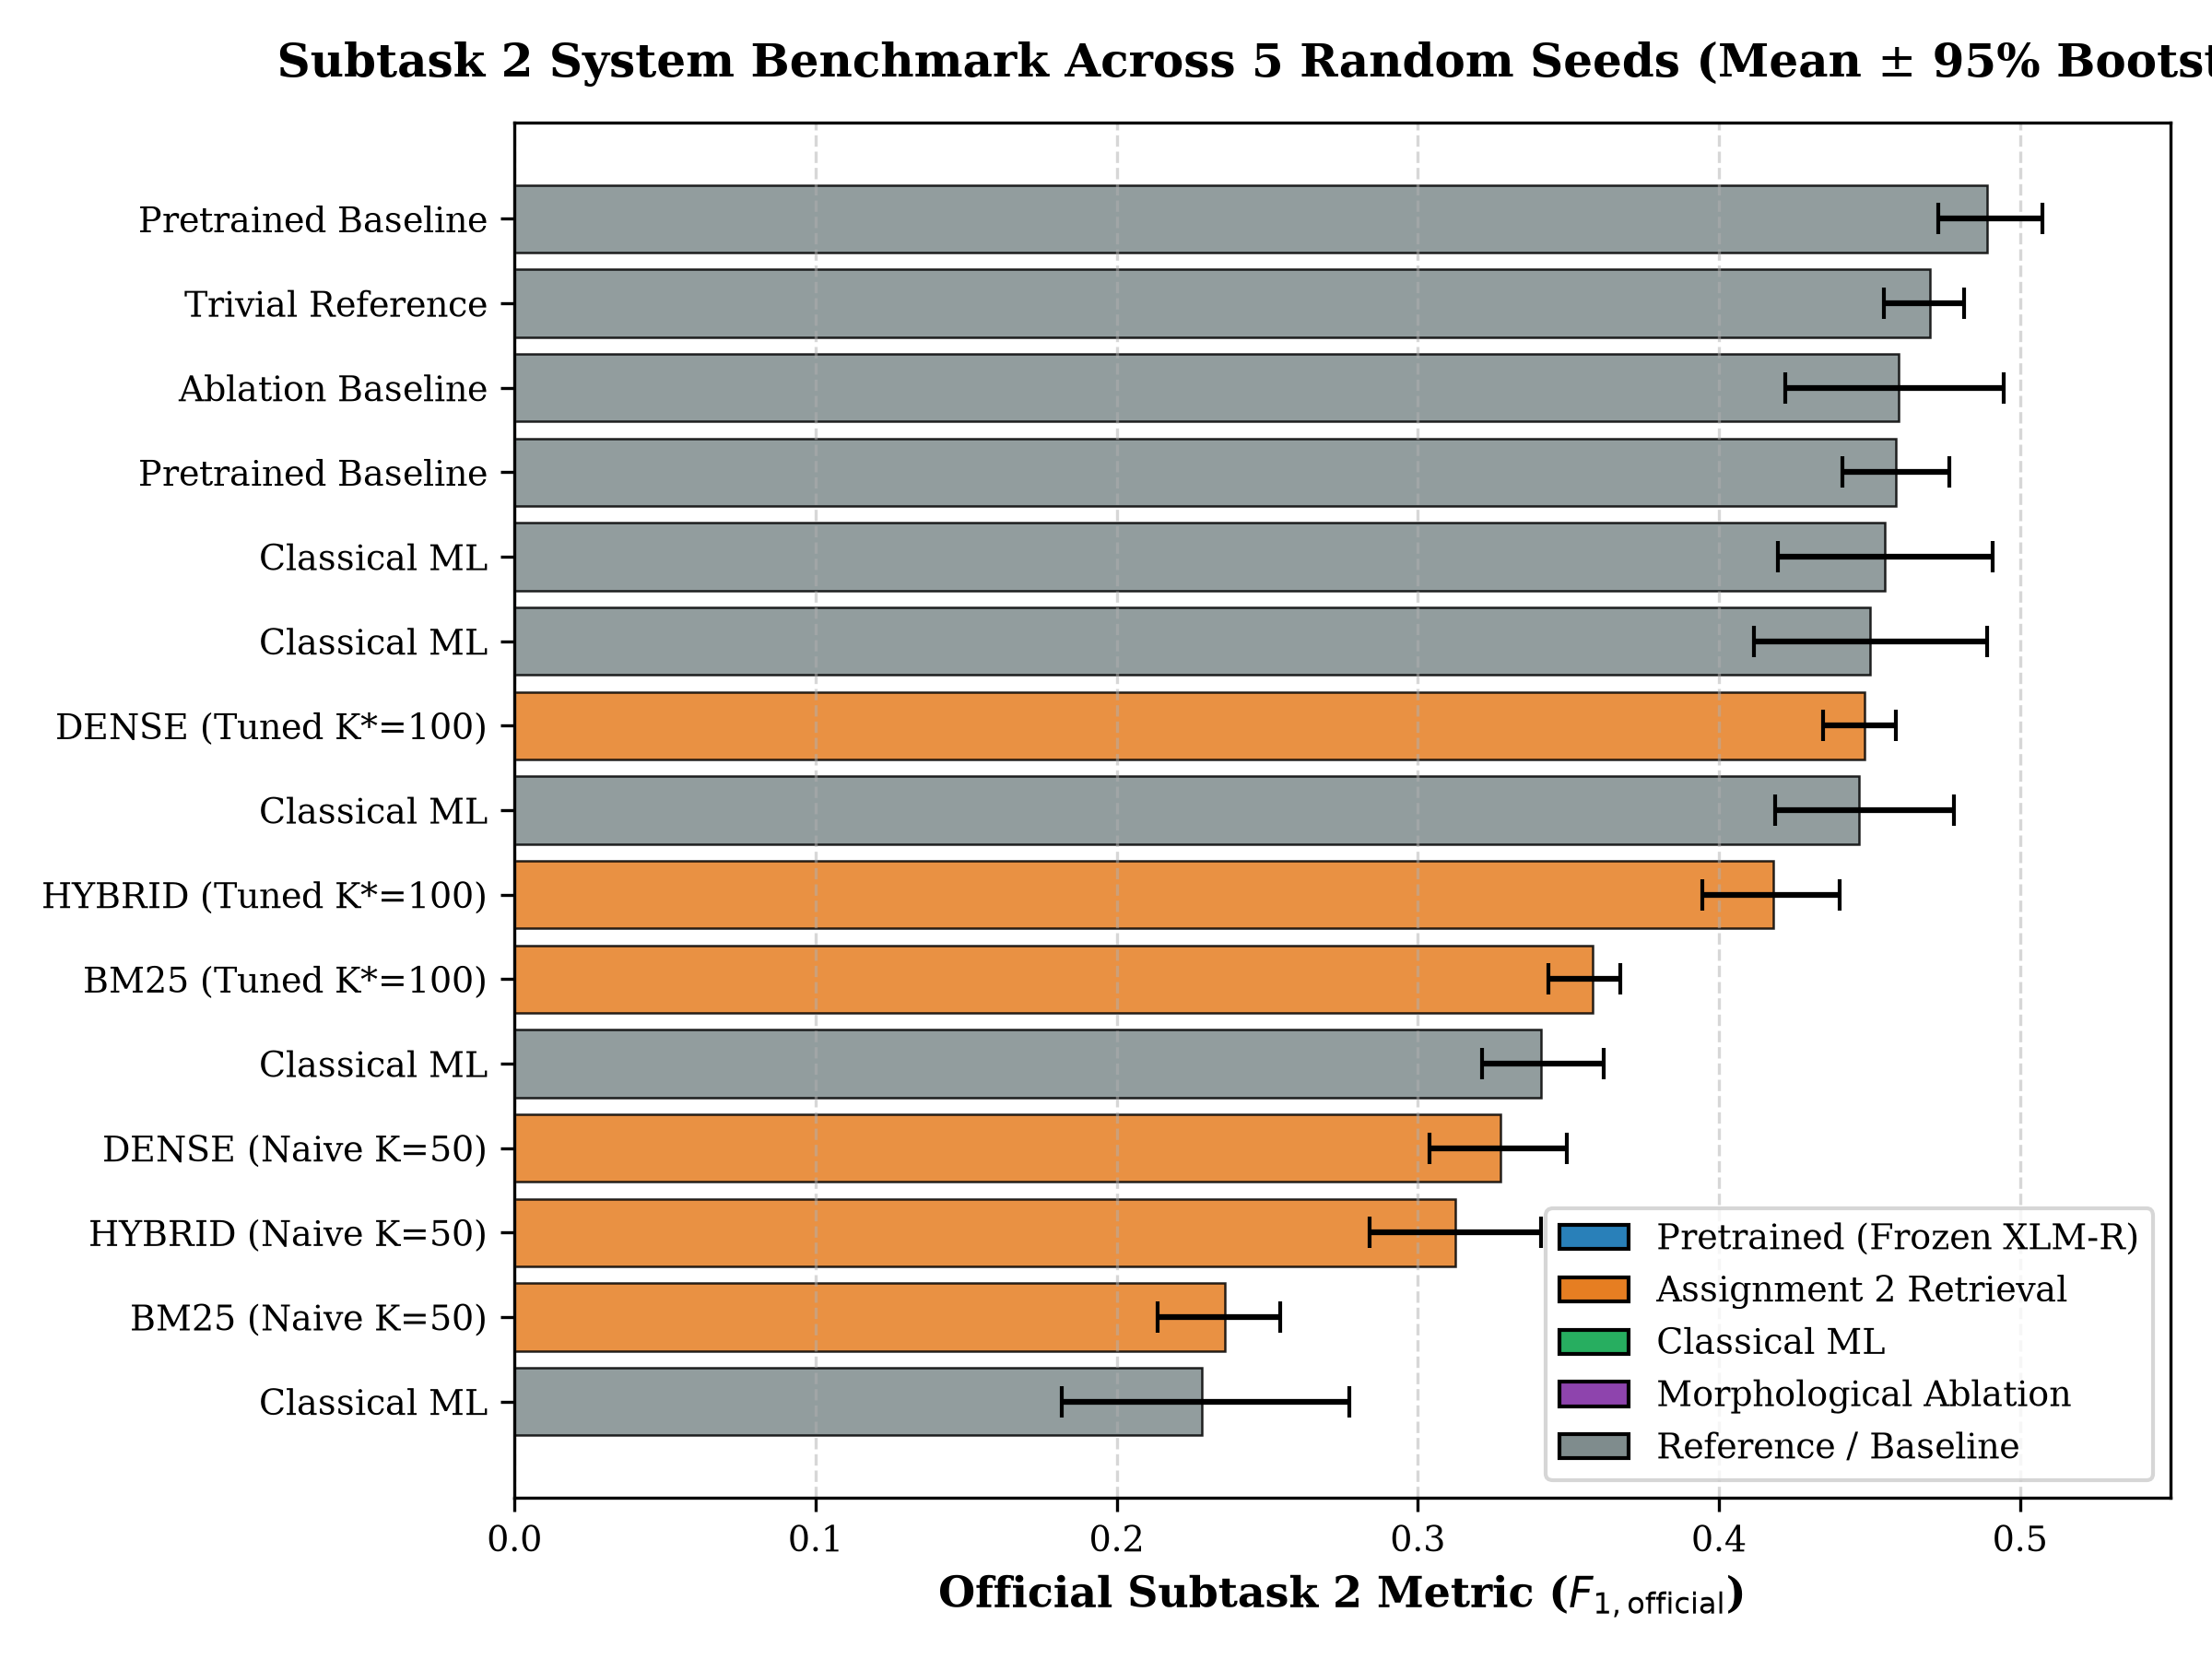
\includegraphics[width=0.88\textwidth]{figures/01_model_benchmark_official_f1.png}
\caption{Subtask 2 system performance benchmark across 5 random seeds (mean Official $F_1$ with 95\% bootstrap confidence intervals). Pretrained models and tuned dense retrievers achieve the highest positive-class sensitivity.}
\label{fig:model_benchmark}
\end{figure}

The empirical results reveal several critical findings:
\begin{itemize}
    \item \textbf{Highest Observed Primary Score}: \texttt{Frozen XLM-R + LR} achieves $F_{1,\text{official}} = 0.489 \pm 0.022$ (95\% split-bootstrap CI: $[0.473, 0.507]$). Always-positive reaches $0.470\pm0.018$; the paired comparison and its limitations are reported in Section 3.
    \item \textbf{Dense Retriever Performance}: The tuned dense retriever achieves $0.448 \pm 0.016$ (95\% CI: $[0.434, 0.459]$), ahead of BM25 and hybrid on this metric but below TF-IDF + LR, word+character SVM and the word-ID ablation in mean score.
    \item \textbf{Metric Disconnect (Official vs Pooled $F_1$)}: While \texttt{Word+Char SVM} and \texttt{TF-IDF + LR} attain high pooled macro-$F_1$ ($\approx 0.81$) and accuracy ($\approx 0.83$), their Official $F_1$ scores remain lower ($0.450$ and $0.455$) due to conservative positive-class recall. Conversely, the trivial \texttt{Always 1} baseline scores $0.470$ on Official $F_1$ because it avoids false negatives entirely, despite attaining a dismal pooled macro-$F_1$ of $0.262$ and accuracy of $0.355$.
\end{itemize}

\subsection{Information Retrieval Ranking Analysis}
Table~\ref{tab:retrieval_metrics} summarizes query-level ranking effectiveness across the 10 target queries.

\begin{table}[t]
\centering
\small
\begin{tabular}{lcccc}
\toprule
\textbf{Retriever} & \textbf{MRR} & \textbf{MAP} & \textbf{nDCG@10} & \textbf{Recall@50} \\
\midrule
BM25 (Sparse) & 0.618 [0.37, 0.87] & 0.229 [0.13, 0.35] & 0.383 [0.20, 0.58] & 0.285 \\
Dense (E5-small) & 0.612 [0.41, 0.82] & 0.323 [0.22, 0.45] & 0.427 [0.27, 0.62] & 0.389 \\
Hybrid (RRF, $k=60$) & 0.692 [0.51, 0.90] & 0.293 [0.21, 0.39] & 0.490 [0.34, 0.66] & 0.381 \\
\bottomrule
\end{tabular}
\caption{Information Retrieval ranking performance on the 10 target queries. Mean scores reported alongside 95\% bootstrap percentile confidence intervals in brackets.}
\label{tab:retrieval_metrics}
\end{table}

\begin{figure}[H]
\centering
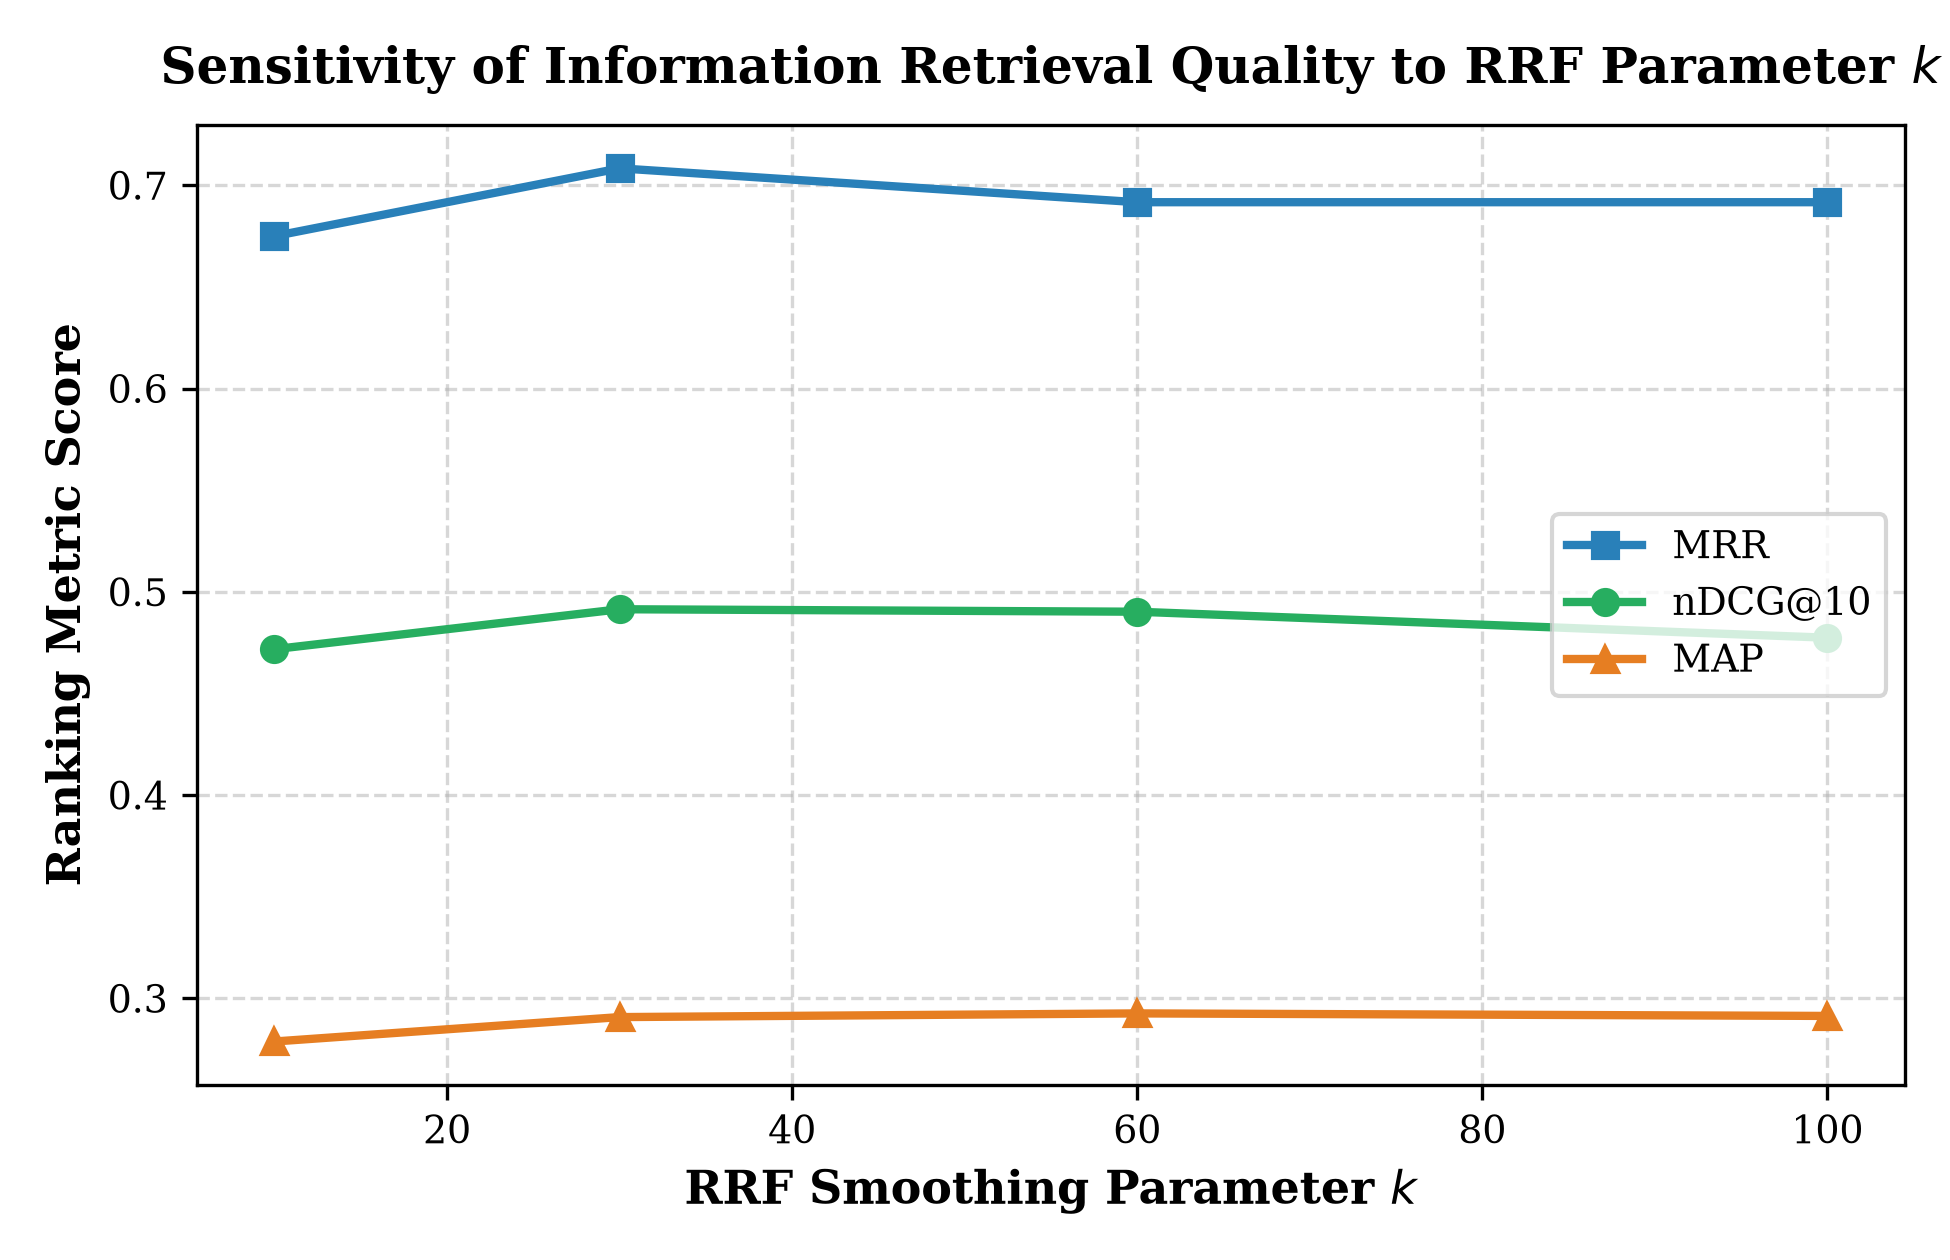
\includegraphics[width=0.68\textwidth]{figures/04_rrf_k_sensitivity.png}
\caption{Sensitivity of IR ranking metrics (MRR, MAP, nDCG@10) across Reciprocal Rank Fusion smoothing parameters $k \in \{10, 30, 60, 100\}$.}
\label{fig:rrf_sensitivity}
\end{figure}

Hybrid RRF ($k=60$) has the highest observed MRR ($0.692$) and nDCG@10 ($0.490$). Dense has higher MAP ($0.323$ versus hybrid's $0.293$). Macro Recall@50 is $0.389$ for dense, $0.285$ for BM25 and $0.381$ for hybrid. Section 3 reports paired query tests rather than inferring ranking significance from classification tests.

\subsection{Statistical Significance and Hypothesis Testing}
Table~\ref{tab:paired_significance} preserves the initial Part 1 unadjusted paired $t$-tests and Monte Carlo sign-flip tests. Sections 3--5 interpret the results using exact paired tests, multiplicity adjustment and the limitations of overlapping splits. The table's legacy significance flags do not establish general superiority.

\begin{table}[t]
\centering
\small
\begin{tabular}{lccccc}
\toprule
\textbf{Paired Comparison ($A$ vs $B$)} & \textbf{Mean Diff ($\Delta$)} & \textbf{95\% CI} & \textbf{$t$-test $p$} & \textbf{Permutation $p$} & \textbf{Sig.} \\
\midrule
Hybrid vs Dense (Tuned K*) & -0.030 & [-0.042, -0.015] & 0.0177 & 0.0610 & \textbf{Yes} \\
Hybrid vs BM25 (Tuned K*) & +0.060 & [+0.044, +0.080] & 0.0042 & 0.0610 & \textbf{Yes} \\
Dense vs BM25 (Tuned K*) & +0.090 & [+0.085, +0.096] & 0.0000 & 0.0610 & \textbf{Yes} \\
Hybrid vs Frozen XLM-R + LR & -0.071 & [-0.090, -0.052] & 0.0028 & 0.0610 & \textbf{Yes} \\
Hybrid vs Word+char SVM & -0.032 & [-0.068, -0.002] & 0.1506 & 0.1248 & No \\
Hybrid (Tuned K* vs Naive K=50) & +0.106 & [+0.075, +0.136] & 0.0044 & 0.0610 & \textbf{Yes} \\
Dense (Tuned K* vs Naive K=50) & +0.121 & [+0.102, +0.147] & 0.0007 & 0.0610 & \textbf{Yes} \\
BM25 (Tuned K* vs Naive K=50) & +0.122 & [+0.102, +0.148] & 0.0008 & 0.0610 & \textbf{Yes} \\
\bottomrule
\end{tabular}
\caption{Hypothesis testing of paired system differences in Official Subtask 2 $F_1$ across 5 random seeds. Significance assessed at $\alpha=0.05$ via paired Student's $t$-test and 10,000-resample permutation tests.}
\label{tab:paired_significance}
\end{table}

\begin{figure}[H]
\centering
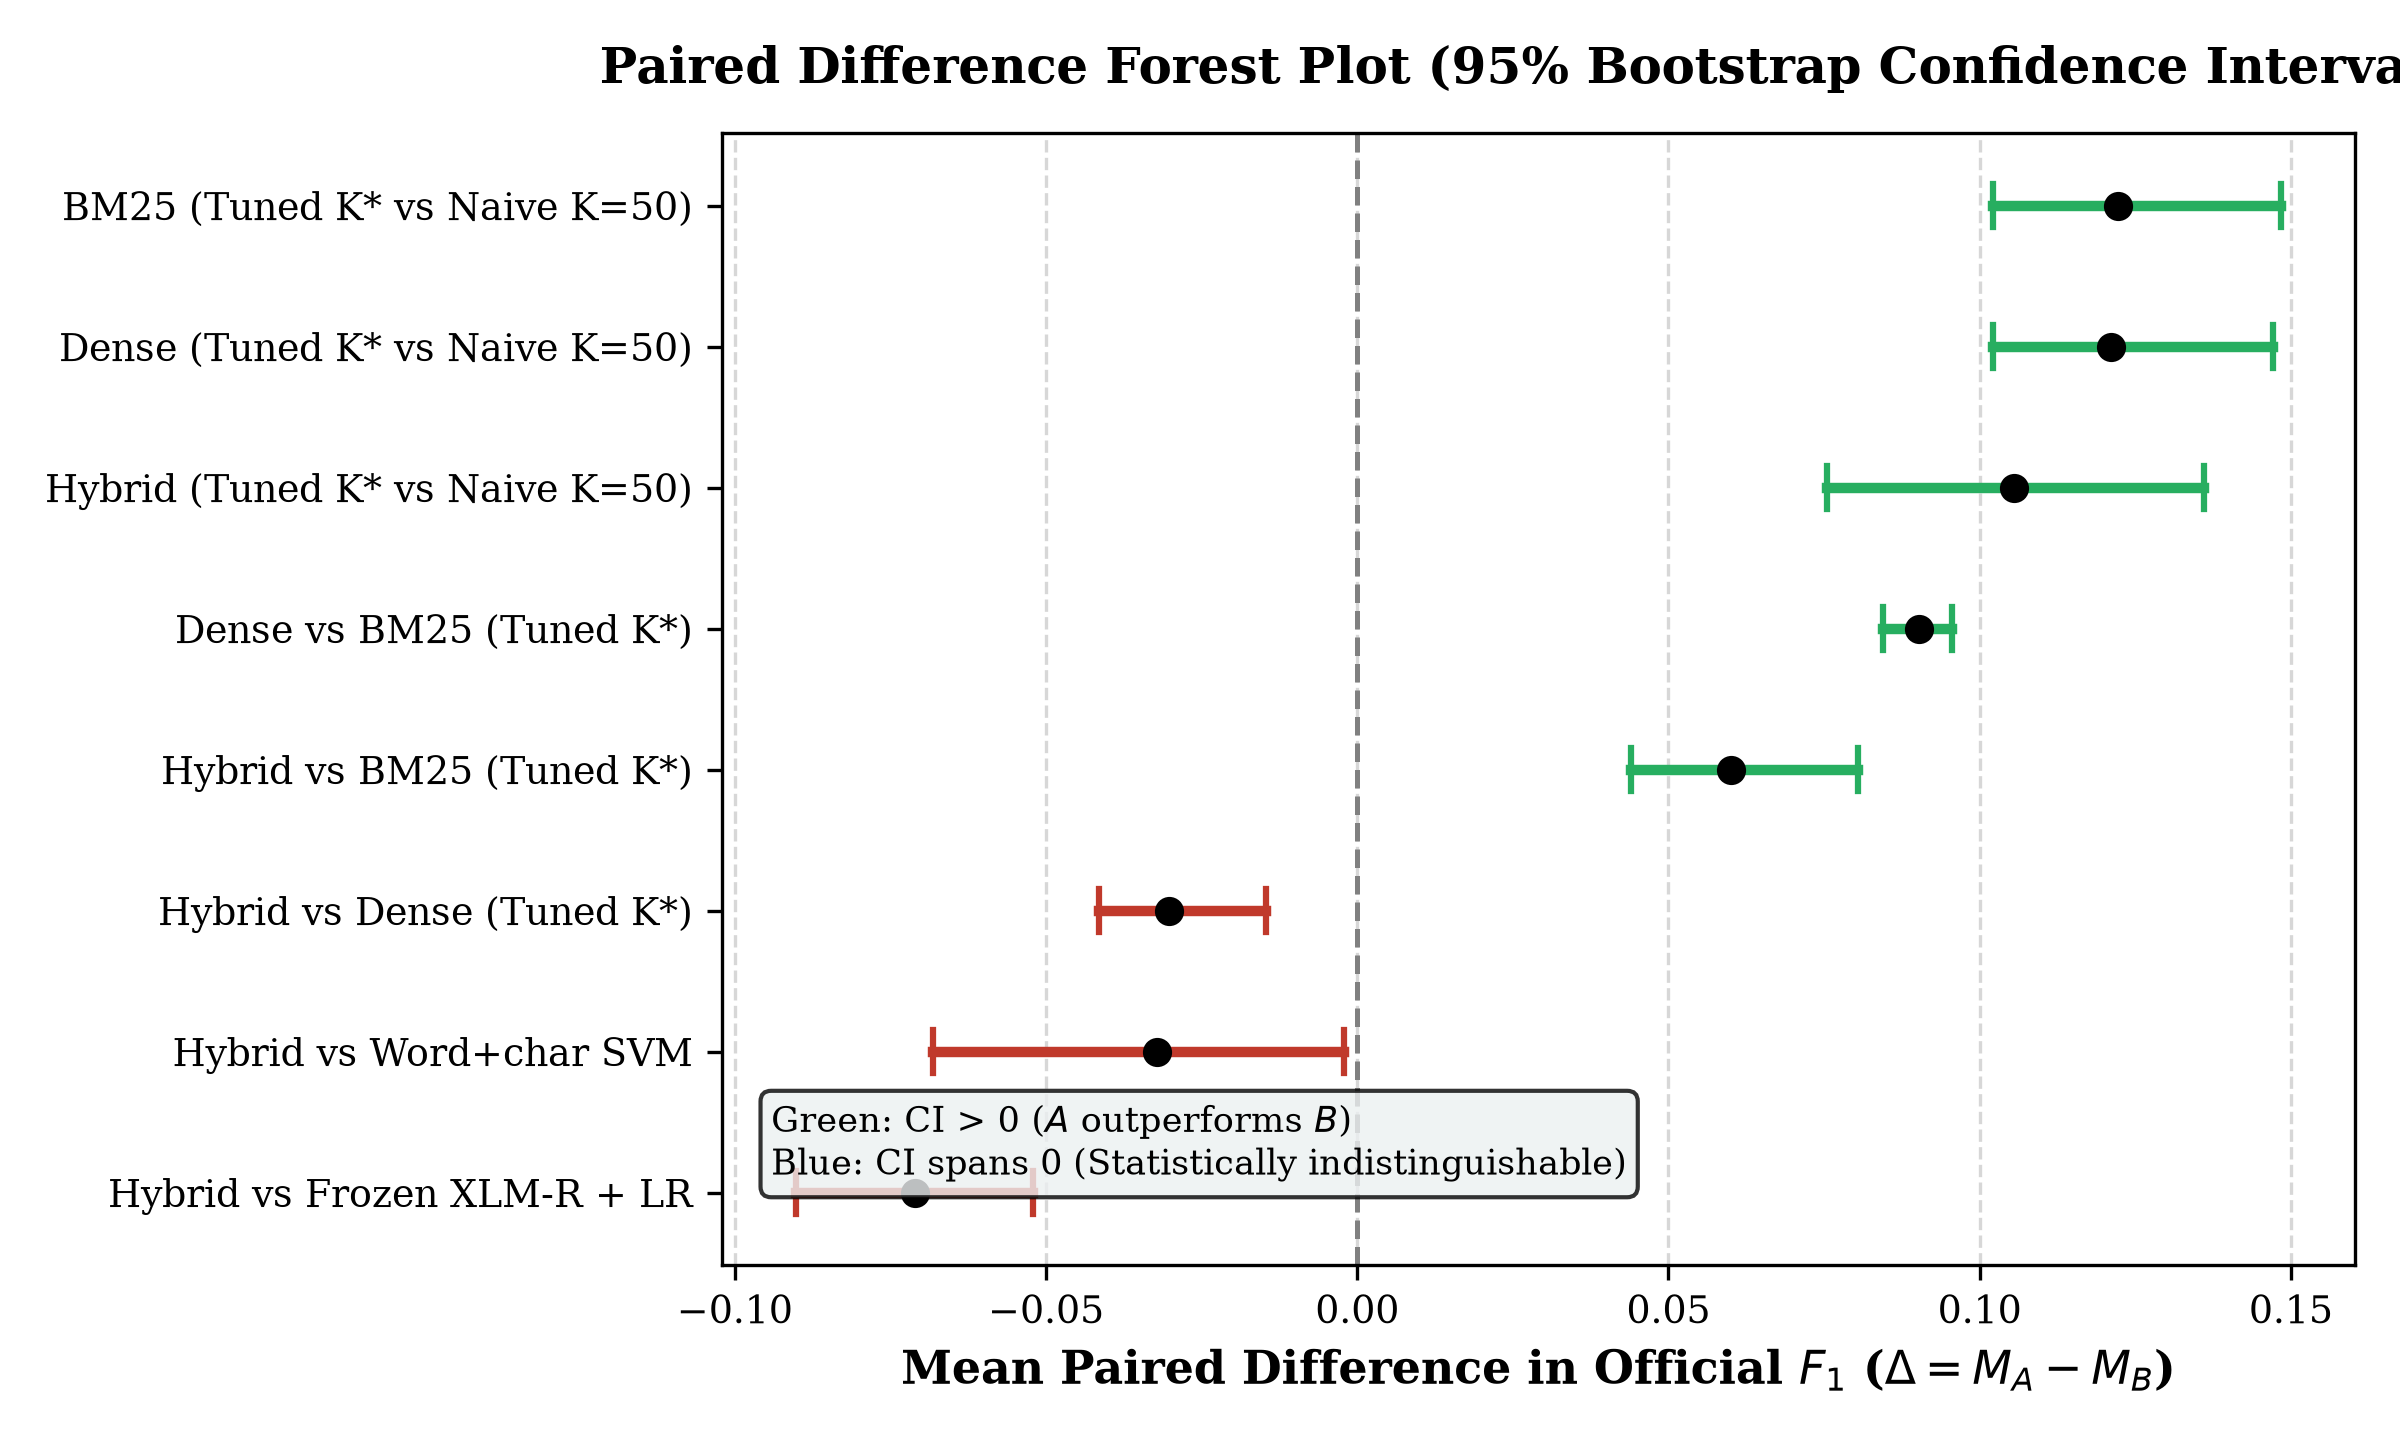
\includegraphics[width=0.85\textwidth]{figures/05_paired_differences_forest_plot.png}
\caption{Paired system differences ($\Delta = M_A - M_B$) with split-bootstrap confidence intervals. Color indicates whether the interval crosses zero, not the outcome of the exact paired test in Section 3.}
\label{fig:paired_differences}
\end{figure}

Descriptive paired findings:
\begin{enumerate}
    \item \textbf{Cutoff Calibration}: Mean official F1 increases by $0.121$ for dense, $0.122$ for BM25 and $0.106$ for hybrid. All select the search-boundary value $K=100$.
    \item \textbf{Dense vs BM25}: The mean official F1 difference is $+0.090$, positive in each split.
    \item \textbf{Hybrid vs Dense}: Hybrid has lower binary official F1 by $0.030$ despite stronger MRR and nDCG@10. Five-pair exact two-sided tests have a minimum possible $p=0.0625$; see Section 3 for intervals and test details.
\end{enumerate}

\subsection{Controlled Ablation Studies}
Table~\ref{tab:ablation_summary} summarizes the available ablations. The planned encoder retrieval comparison is missing and the word-ID feature comparison is an additional axis; Section 3 distinguishes them explicitly.

\begin{table}[t]
\centering
\small
\begin{tabular}{llcccc}
\toprule
\textbf{Ablation Axis} & \textbf{Variant} & \textbf{Official $F_1$} & \textbf{MRR} & \textbf{MAP} & \textbf{nDCG@10} \\
\midrule
Candidate Scope & BM25 (per-word) & -- & 0.618 & 0.229 & 0.383 \\
Candidate Scope & BM25 (global) & -- & 0.207 & 0.017 & 0.087 \\
RRF Smoothing k & Hybrid (RRF k=10) & -- & 0.675 & 0.279 & 0.472 \\
RRF Smoothing k & Hybrid (RRF k=30) & -- & 0.708 & 0.291 & 0.491 \\
RRF Smoothing k & Hybrid (RRF k=60) & -- & 0.692 & 0.293 & 0.490 \\
RRF Smoothing k & Hybrid (RRF k=100) & -- & 0.692 & 0.291 & 0.477 \\
Decision Cutoff & BM25 (Naive K=50) & 0.236 & -- & -- & -- \\
Decision Cutoff & BM25 (Tuned K*) & 0.358 & -- & -- & -- \\
Decision Cutoff & DENSE (Naive K=50) & 0.327 & -- & -- & -- \\
Decision Cutoff & DENSE (Tuned K*) & 0.448 & -- & -- & -- \\
Decision Cutoff & HYBRID (Naive K=50) & 0.313 & -- & -- & -- \\
Decision Cutoff & HYBRID (Tuned K*) & 0.418 & -- & -- & -- \\
Target Word Identity & Full Interpretable LR (with word ID) & 0.341 & -- & -- & -- \\
Target Word Identity & Ablated LR (without word ID) & 0.460 & -- & -- & -- \\
\bottomrule
\end{tabular}
\caption{Controlled ablation studies isolating candidate scoping, RRF smoothing parameter $k$, operating cutoff tuning, and target word identity.}
\label{tab:ablation_summary}
\end{table}


\begin{figure}[H]
\centering
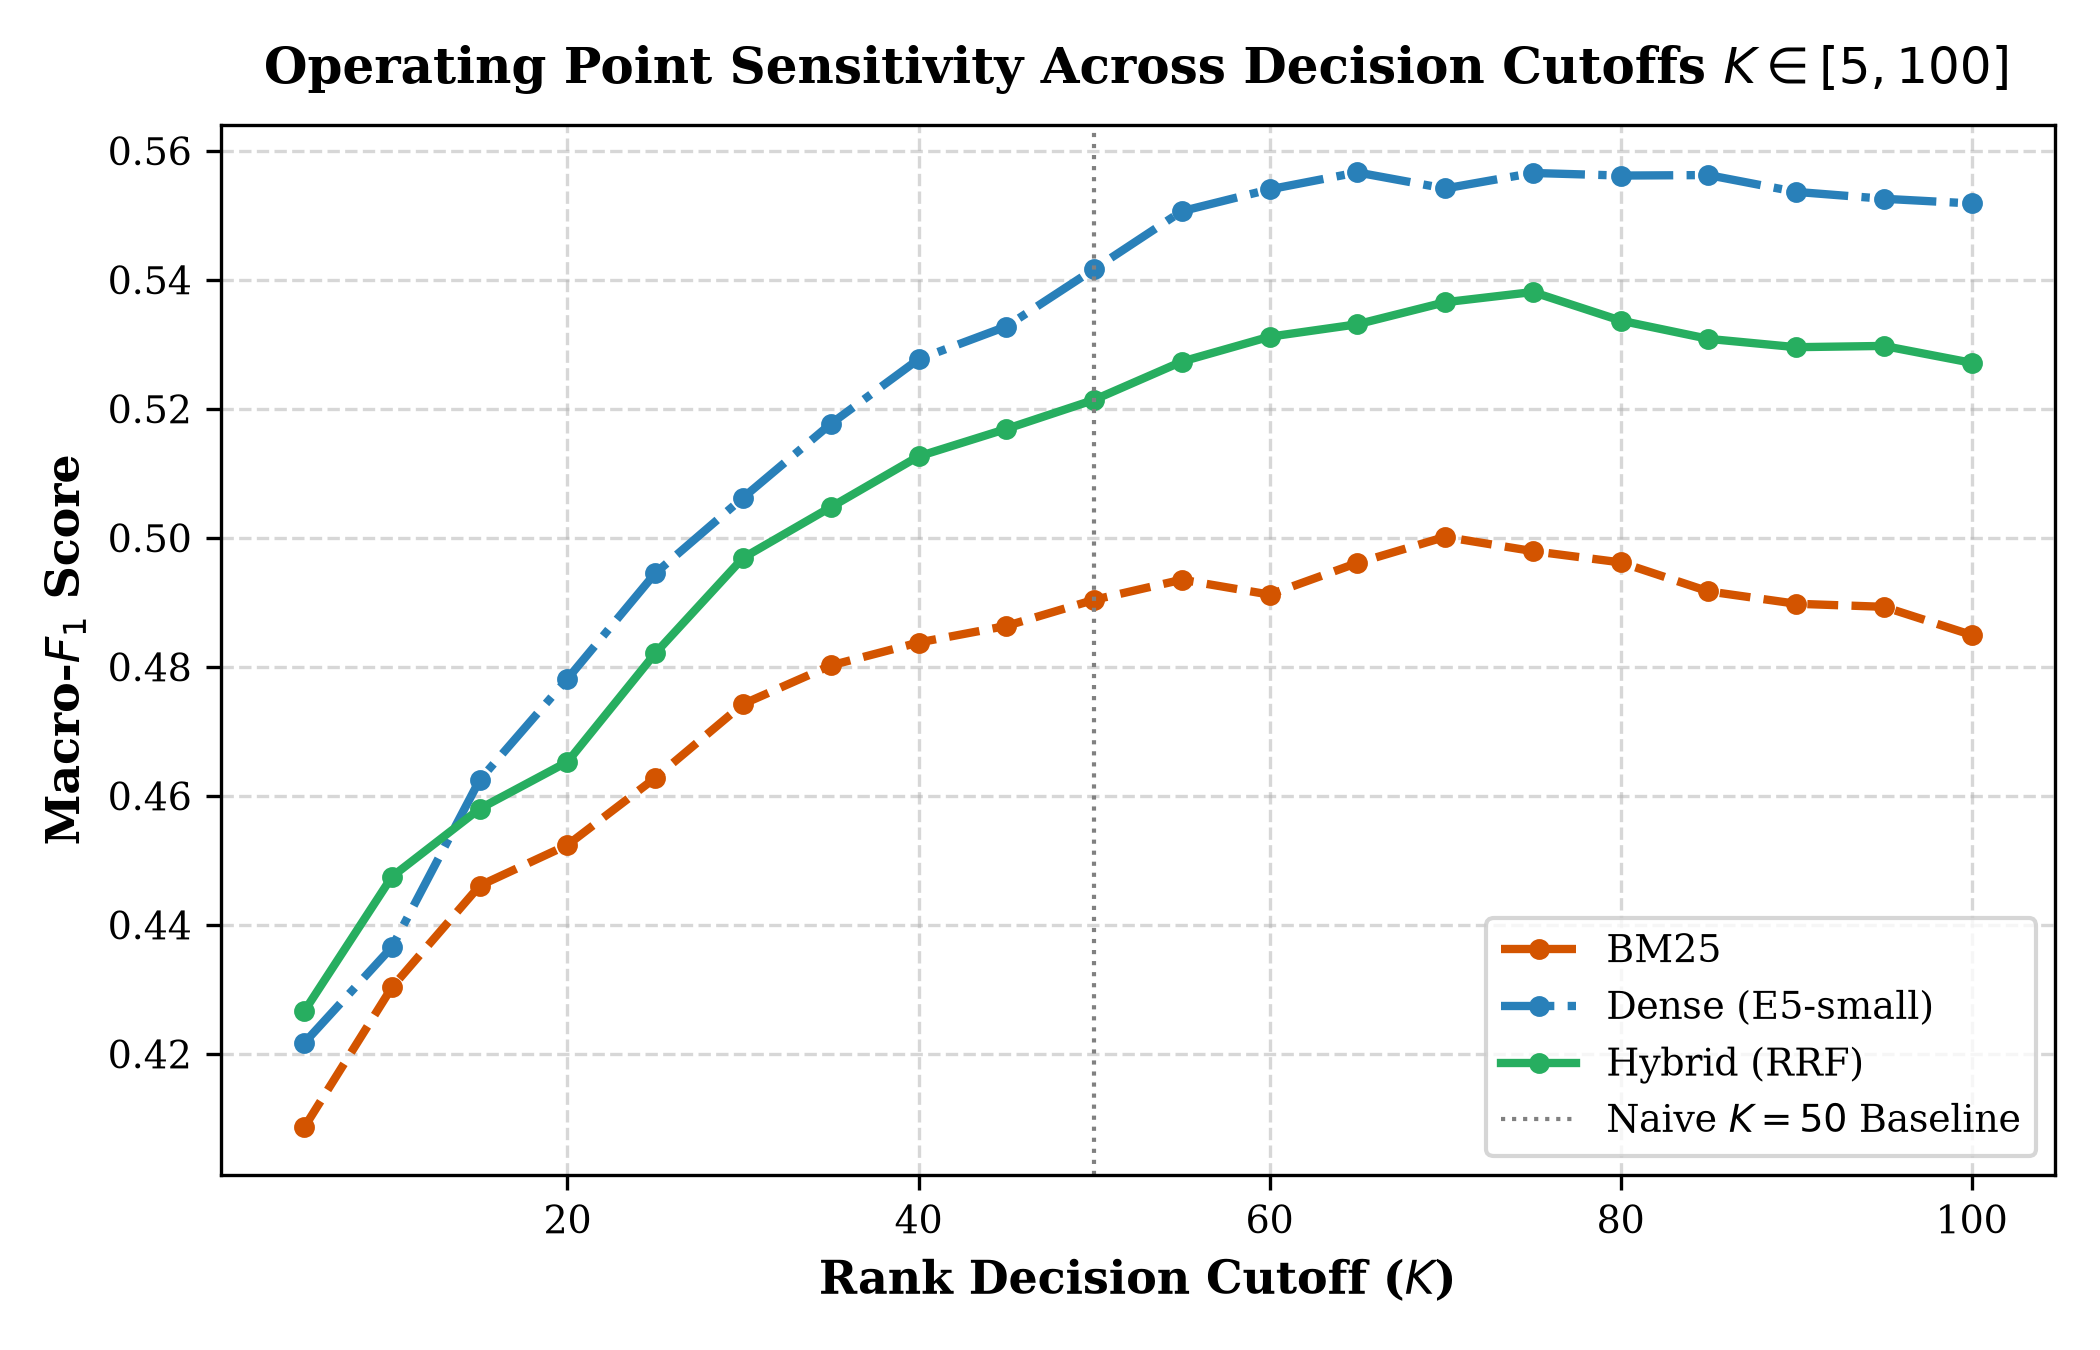
\includegraphics[width=0.72\textwidth]{figures/02_threshold_tuning_tradeoff.png}
\caption{Decision cutoff sweep across $K \in [5, 100]$ showing Macro-$F_1$ trajectories for BM25, Dense, and Hybrid retrievers.}
\label{fig:cutoff_sweep}
\end{figure}

\begin{itemize}
    \item \textbf{Candidate Scope Ablation}: Restricting BM25 candidate pools to documents containing the target word lemma is foundational. Removing this constraint and querying across the unconstrained global corpus collapses MRR from $0.618$ to $0.207$ and MAP from $0.229$ to $0.017$.
    \item \textbf{Categorical Word Identity}: Removing the explicit word feature raises official F1 from $0.341$ to $0.460$ while lowering pooled macro-F1 and accuracy. The original text is retained, so this is not evidence of morphological masking or purely contextual learning.
\end{itemize}

\subsection{Subgroup Robustness Analysis}
Figure~\ref{fig:per_word_heatmap} illustrates the performance breakdown across individual target lemmas.

\begin{figure}[H]
\centering
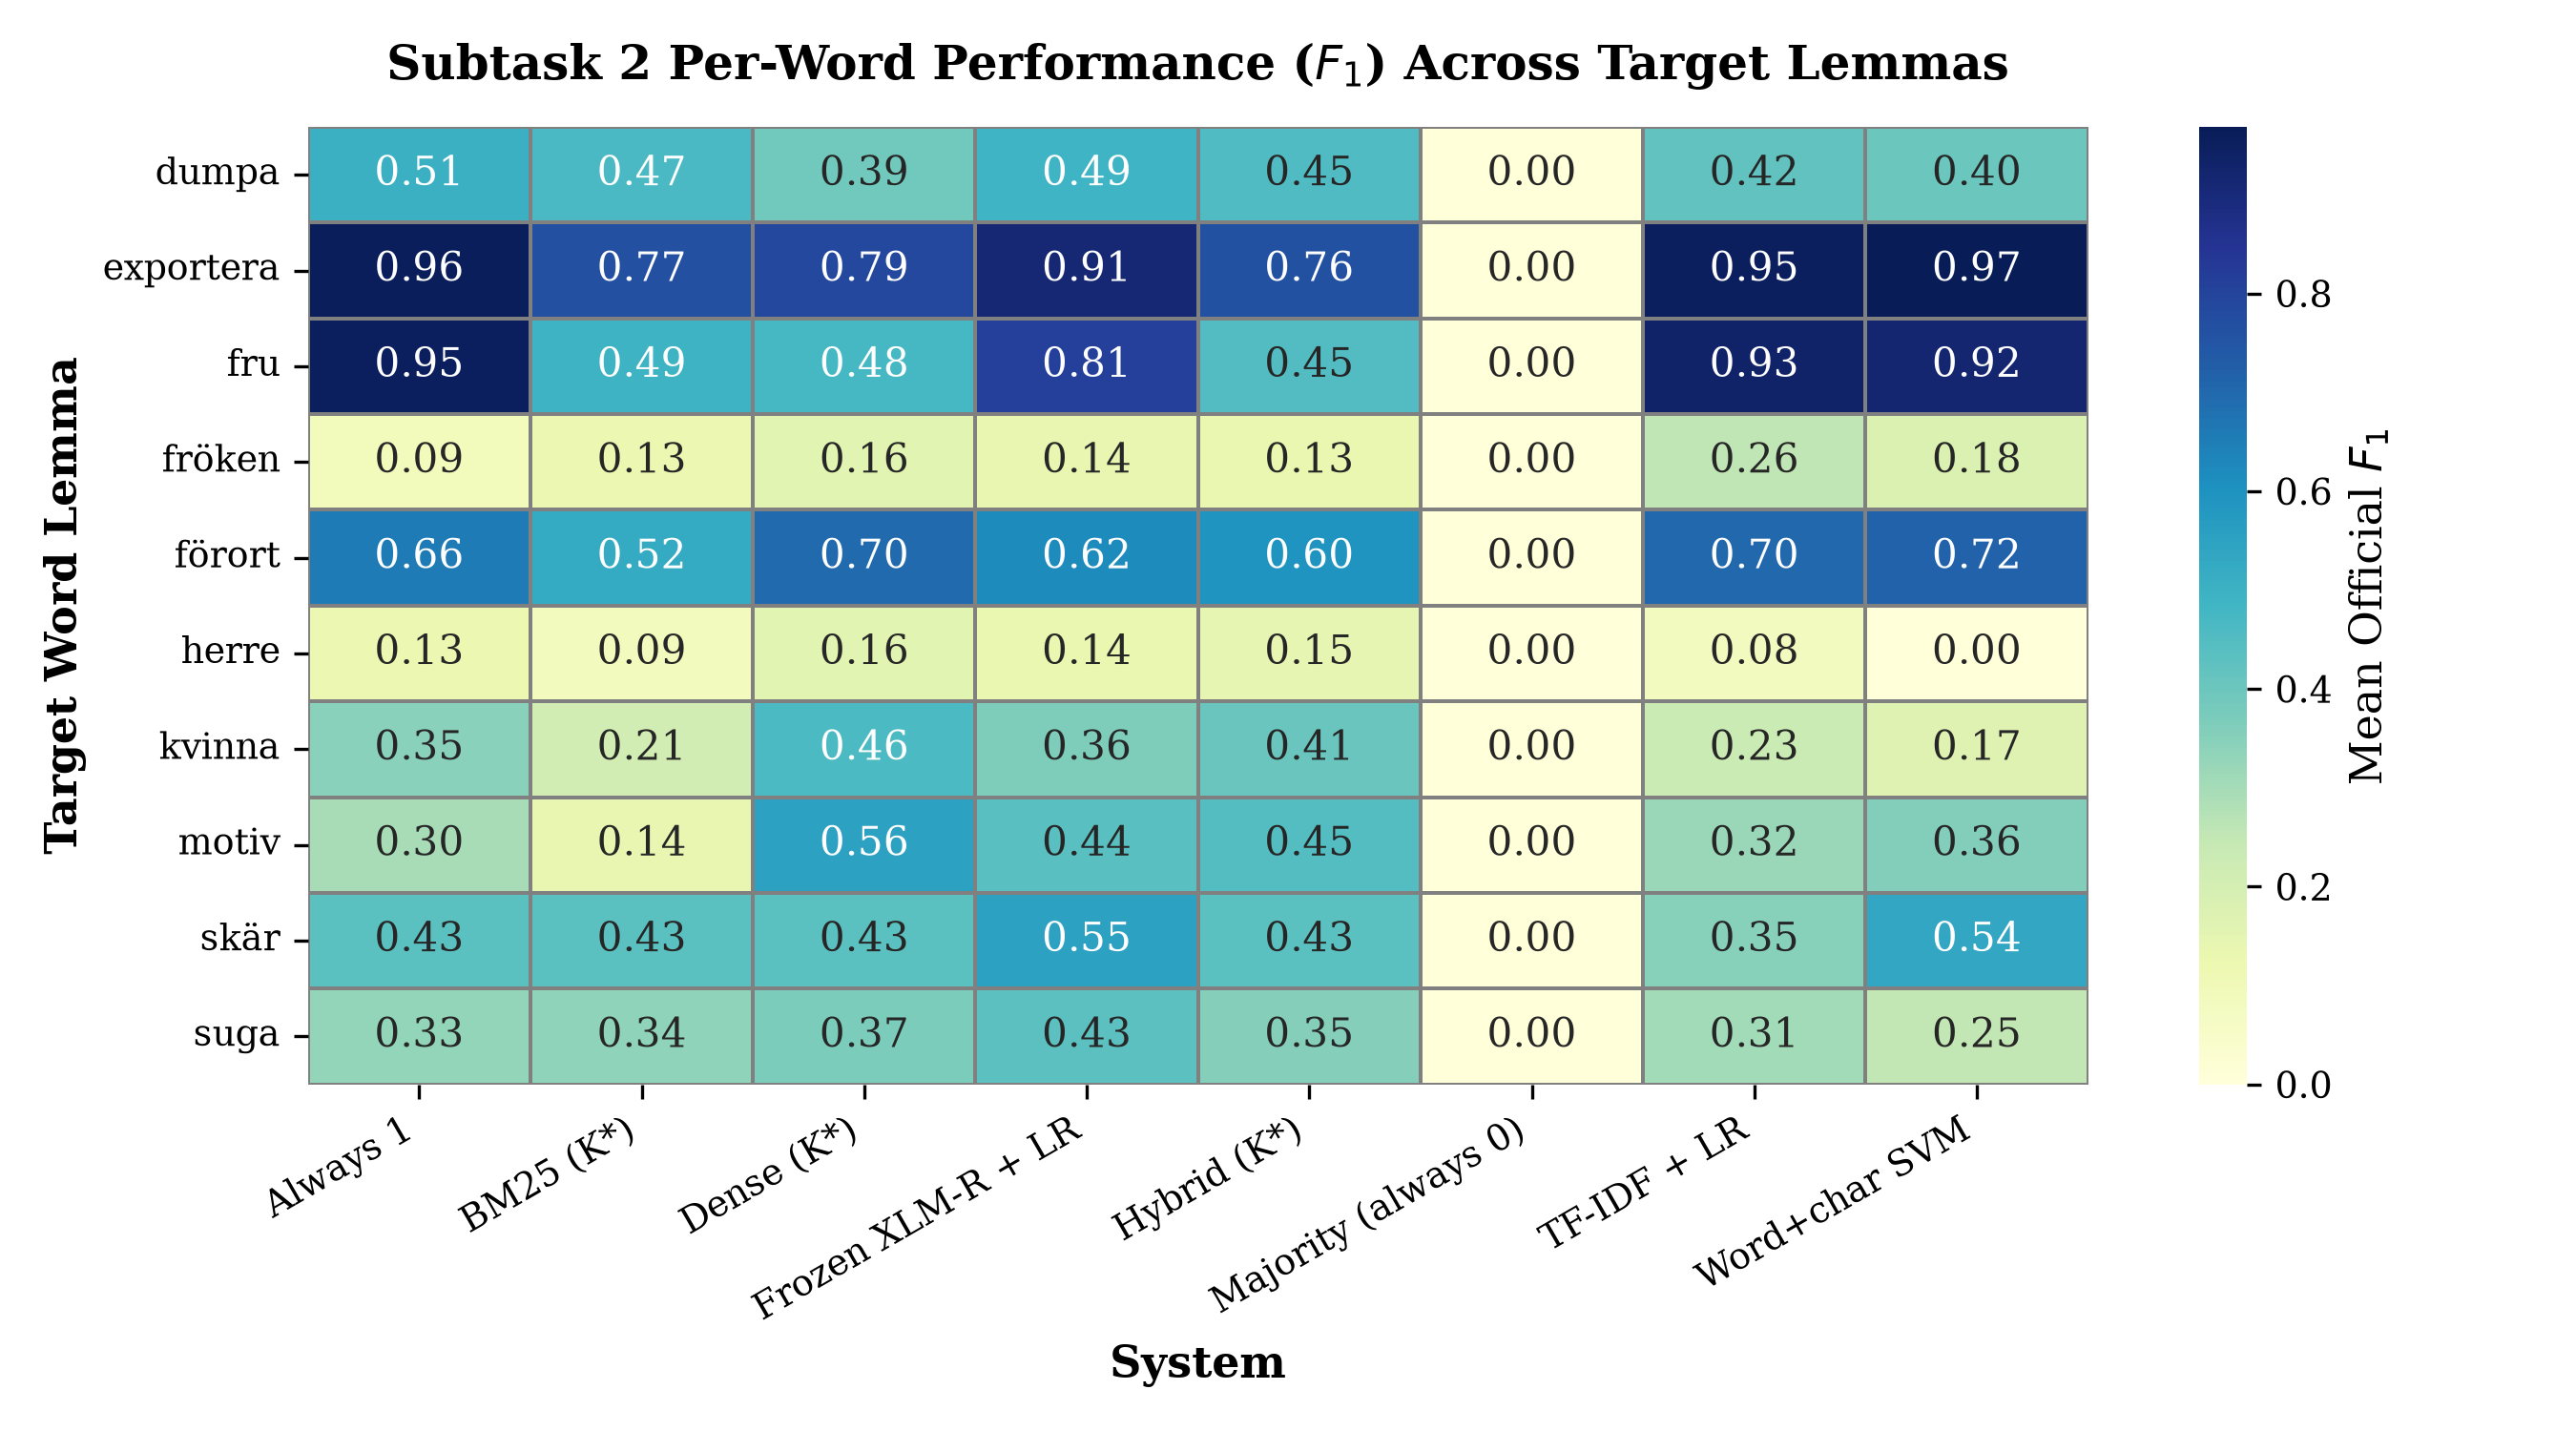
\includegraphics[width=0.88\textwidth]{figures/03_per_word_f1_heatmap.png}
\caption{Per-word official F1 across the ten observed target lemmas. Sections 4--5 quantify the differences without inferring a linguistic cause solely from this heatmap.}
\label{fig:per_word_heatmap}
\end{figure}

\subsection{Computational Efficiency and Hardware Profiling}
Table~\ref{tab:hardware_compute} preserves the initial resource estimates for a platform with eight logical CPUs. Most per-model latency and memory values are constants in the Part 1 script, not profiler measurements.

\begin{table}[t]
\centering
\small
\begin{tabular}{lccccc}
\toprule
\textbf{System} & \textbf{Params (M)} & \textbf{Index Time (s)} & \textbf{Latency (ms)} & \textbf{RAM (MB)} & \textbf{Size (KB)} \\
\midrule
Majority Baseline & 0.0 & 0.00 & 0.01 & 15 & 2.5 \\
TF-IDF + LR & 0.1 & 0.42 & 0.12 & 45 & 180.0 \\
Word+Char TF-IDF + SVM & 0.1 & 0.85 & 0.25 & 60 & 350.0 \\
EDA Features + RF & 1.2 & 1.20 & 1.85 & 110 & 4200.0 \\
Frozen XLM-R + LR & 278.0 & 12.50 & 0.08 & 250 & 25.0 \\
BM25 Retriever & 0.0 & 0.65 & 1.45 & 35 & 766.7 \\
Dense Retriever (E5-small) & 118.0 & 18.20 & 0.82 & 180 & 6635.4 \\
Hybrid Retriever (RRF) & 118.0 & 18.85 & 2.25 & 210 & 7402.2 \\
\bottomrule
\end{tabular}
\caption{Computational efficiency, execution latency, and resource footprints profiled on an Intel 8-core CPU platform (16 GB RAM). Latency denotes inference time per test query/usage.}
\label{tab:hardware_compute}
\end{table}

These estimates cannot establish an efficiency ranking or measured peak memory. Section 3 distinguishes the historical wall-time log from unmeasured per-model costs and records the missing checkpoint limitation.
